\documentclass{../../../../fal_assignment}
\graphicspath{ {../../../../} }

\usepackage{url}
\usepackage{graphicx}
\usepackage{amsmath}
\usepackage{varwidth}
\usepackage{xcolor}
\usepackage{algorithm}
\usepackage{algpseudocode}
\usepackage{listings}
\lstset{
	basicstyle=\footnotesize\ttfamily,
	tabsize=4,
	showstringspaces=false,
	breaklines=true,
	prebreak={\space\hbox{\textcolor{Gray}{$\hookleftarrow$}}},
	language=C++
}
\usepackage{enumitem}

\usepackage{tikz}
\usetikzlibrary{shapes.geometric, arrows}

\tikzstyle{flowchartnode} = [rectangle, minimum height=0.8cm, text centered, text width=3cm, draw=black, font=\small]
\tikzstyle{startstop} = [flowchartnode, rounded corners=0.4cm]
\tikzstyle{process} = [flowchartnode]
\tikzstyle{io} = [flowchartnode, trapezium, trapezium left angle=70, trapezium right angle=110, text width=2cm]
\tikzstyle{decision} = [flowchartnode, diamond, aspect=2, text width=2cm]
\tikzstyle{arrow} = [thick,->,>=stealth]

\title{COMP140 Worksheet B: Fractals}
\author{Brian McDonald \& Ed Powley}
\module{COMP140}

\begin{document}

\maketitle

In this worksheet, you will use the SDL2 library (\url{https://www.libsdl.org/index.php}) to write a program to generate and display a fractal; see Figure~\ref{fig:mandelbrot}.
This fractal colours each pixel of the image according to an iterated mathematical formula, as described below.
The following GitHub repository contains a project named \texttt{Fractal} for you to build upon.

\url{https://github.com/Falmouth-Games-Academy/comp140-worksheetB}

This contains code to create and display a random image; you will implement the calculations to generate the fractal.

\begin{figure}[!h]
	\begin{center}
		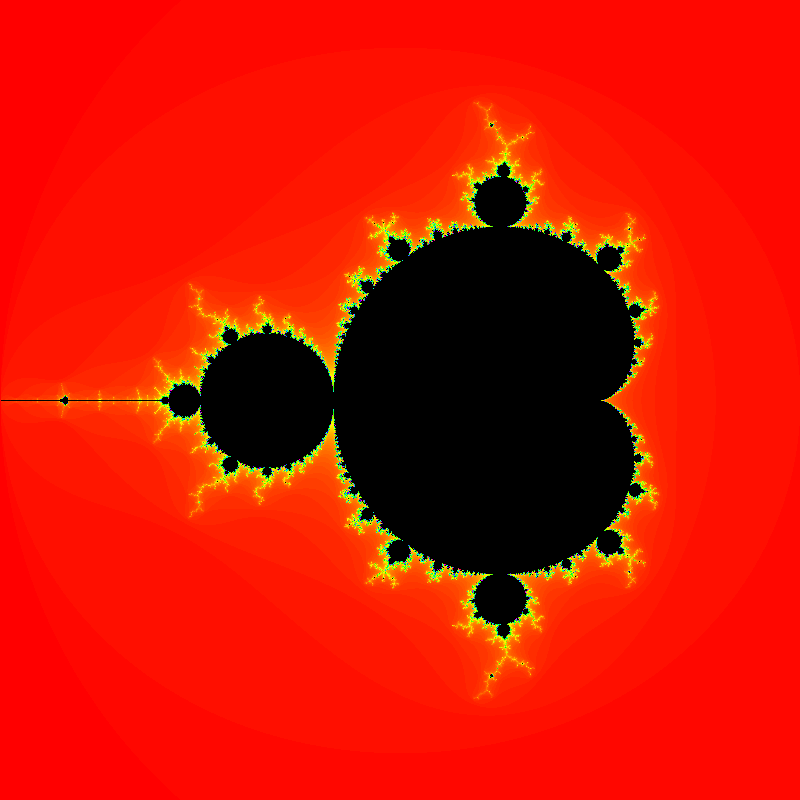
\includegraphics[width=0.6\textwidth]{mandelbrot.png}
	\end{center}
	\caption{An example of a fractal}
	\label{fig:mandelbrot}
\end{figure}

\section{} \label{core-c-first}

To generate an interesting fractal, the on-screen $x$ and $y$ coordinates must first be rescaled.
In the skeleton project the pixel coordinates range from $0$ to $800$,
whereas the fractal is most interesting in the region $-2 \leq x \leq 1$ and $-1.5 \leq y \leq 1.5$.

Let $p_x$ be the $x$ coordinate of the pixel. This can be remapped into the range $x_{\text{min}}$ to $x_{\text{max}}$ using the following formula:
\begin{equation*}
x_0 = \frac{p_x}{\text{image.width}} \times \left( x_{\text{max}} - x_{\text{min}} \right) + x_{\text{min}}
\end{equation*}
The $y$ coordinate can be remapped using a similar formula.

\textbf{Implement} the above calculations for the $x$ and $y$ coordinates, at the indicated parts of \texttt{Fractal.cpp}.

\section{} \label{core-c-last}

The fractal set is based on the following sequence of numbers. Let $x_0$ and $y_0$ be the coordinates of a point in the image.
Then the sequence $x_1, y_1, x_2, y_2, x_3, y_3, \dots$ is defined\footnote{%
	If you are familiar with complex numbers, you may notice that this is equivalent to $z_{j+1} = z_j^2 + z_0$, where $z_j = x_j + y_j i$.
} recursively for $i = 0, 1, 2, 3, \dots$ by:

\begin{align*}
x_{i+1} &= (x_i)^2 - (y_i)^2 + x_0 \\
y_{i+1} &= (2 \times x_i \times y_i) + y_0 \\
\end{align*}

The points are coloured according to the \emph{smallest} value of $i$ for which $(x_i)^2 + (y_i)^2 \geq 4$.
If such a value of $i$ is not found after a large number of iterations (for example $i=200$), the pixel is coloured black.

\textbf{Implement} an algorithm which performs the above computation, determining the smallest value of $i$
for which $(x_i)^2 + (y_i)^2 \geq 4$ and selecting the appropriate pixel colour.

Implement the algorithm in \texttt{main.cpp} so that the program generates the fractal (Figure~\ref{fig:mandelbrot}) when it is run.

\section*{Submission instructions}

You should submit this project as part of the final coursework submission.
	
\section*{Marking criteria}
	
	Remember that \textbf{it is better to submit incomplete work than to submit nothing at all}. 
	
	To demonstrate \textbf{basic competency}, complete the following:
	\begin{itemize}
		\item \textbf{Timely Submission:} Obtain the marks for timely submission, you must submit (as a GitHub pull request).
		As with other worksheets, you may resubmit after these deadlines in order to collect extra correctness or quality marks.
		This is awarded as long as you submit \emph{something} for each part by the deadline,
		even if your submission has bugs or other issues.
		\item Some evidence of emerging innovation and/or creativity in the design of the controller and game.
	\end{itemize} 
	
	To demonstrate \textbf{basic proficiency}, complete the following:
	\begin{itemize}
		\item \textbf{Achieve basic competency}
		\item \textbf{Complete} Algorithm \ref{core-c-first}. \textbf{Note:} You will not be penalised for trivial errors which do not
		affect the overall functioning of your programs
		\item Appropriate use of GitHub, with descriptive commit messages 
		\item Comments are used where appropriate, and are well written.
		\item Little evidence of emerging innovation and/or creativity in the design of the controller and game.
	\end{itemize}
	
	To demonstrate \textbf{novice competency}, complete the following:
	\begin{itemize}
		\item Achieve \textbf{basic proficiency}
		\item \textbf{Complete} Algorithm \ref{core-c-last}. \textbf{Note:} You will not be penalised for trivial errors which do not
		affect the overall functioning of your programs
		\item Your code is well formatted. Variable and function names are clear and descriptive.
		\item Much evidence of emerging innovation and/or creativity in the design of the controller and game.
	\end{itemize}
	
	To demonstrate \textbf{novice proficiency}, complete the following:
	\begin{itemize}
		\item Achieve \textbf{novice competency}
		\item \textbf{Research} a different fractal
		\item Considerable evidence of mastery of innovative and creative practice in the design of the controller and game.
	\end{itemize}
	
	To demonstrate \textbf{professional competency}, complete the following:
	\begin{itemize}
		\item Achieve \textbf{novice proficiency}
		\item \textbf{Implement} a new fractal and allow the user to choose what fractal to generate
		\item Significant evidence of mastery of innovative and creative practice  in the design of the controller and game.
	\end{itemize}
	
	
\end{document}
